\section{Versuchsaufbau}
\label{sec:Versuchsaufbau}
Die wichigsten Bausteine dieses Versuches sind der Lautsprecher und das Mikrofon, sowie 
die damit verbunden Steuerelektronik. Sie werden für jeden Versuchsteil benötigt.
Innerhalb dieser Steuerelektronik befindet sich ein Frequenz-Spannungskonverter, 
der es ermöglicht Frequenzspektren auf einem Oszilloskop oder COmputer zu visualisieren.
Auf dem Computer erfolgt die Darstellung mit dem Programm SpectrumSLC.
Der Lautsprecher ist mit einem Sinusgenreator verbunden, üder den die passenden 
Frequenzen erzeugt werden können.

\begin{figure}
    \centering
    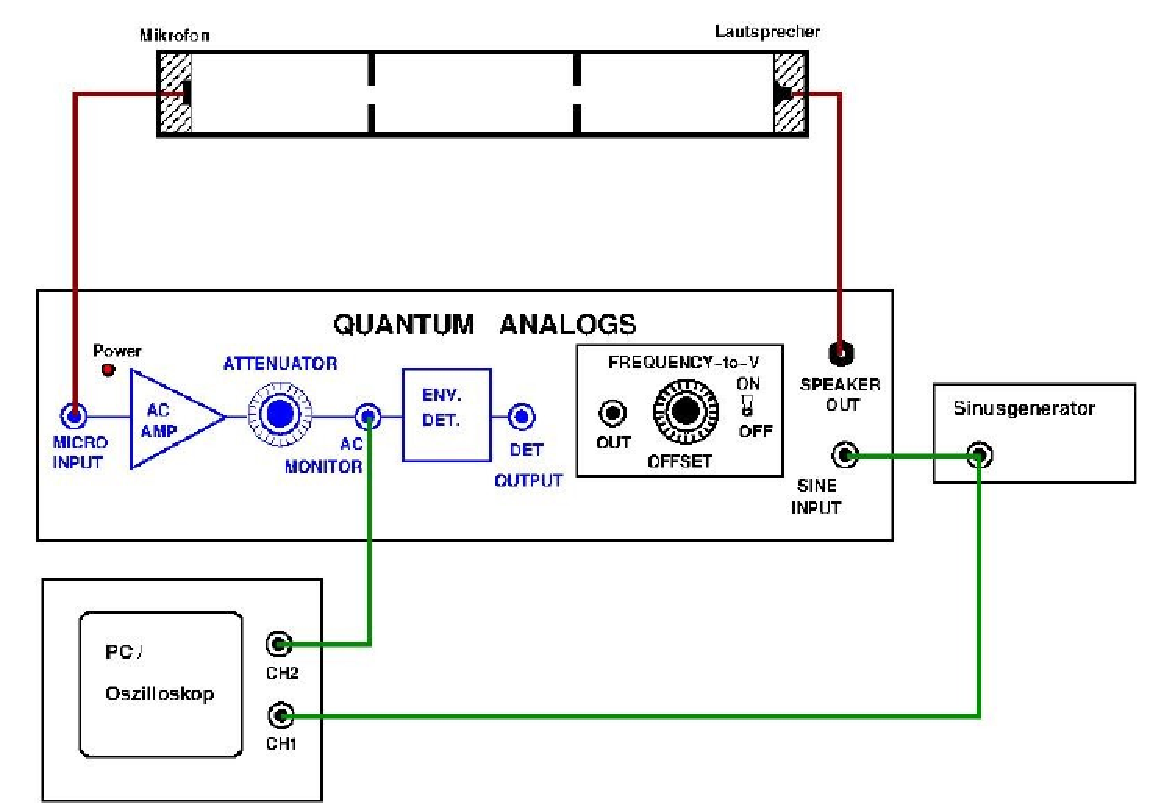
\includegraphics[width=0.9\textwidth]{figure/Schaltung.pdf}
    \caption{Diese Abbildung zeigt, die in diesem Versuch verwendete Schaltung. Im 
    oberen Teil der Abbildung ist eine Metallschiene zu sehen, auf welcher 
    Aluminumzylinder eingespannt und mit einer Frequenz durchlaufen 
    werden können. An dieser Stelle kann alternativ auch der Kugelresonator 
    bzw. die Kombination aus zwei Kugelresonatoren eingebaut werden. 
    Rechts im Bild befindet sich der Sinusgenreator, welcher die 
    Schallfrequenzen erzeugen kann. Links unten befindet sich das 
    Zweikanaloszilloskop oder alternativ ein Computer mit dem Programm
    SpectrumSLC. Die Schnittstelle Quantum Analogs verbindet alle 
    Komponenten in der richtigen Reihenfolge miteinnader. An diesem 
    Gerät können auch zusätziche Einstellungen wie Signalverstärkungen 
    oder -verschwächerungen vorgenommen werden
    \cite{sample}.}
\end{figure}

\newpage
Für unterschiedliche Versuchsteile werden verschiedene Hohlraumresonatoren benötigt:
\begin{itemize}
    \item eindimensionaler Festkörper:
        \begin{itemize}
            \item Aluminiumzylinder der Längen: $\SI{12,5}{\milli\meter}$, $\SI{50}{\milli\meter}$ und $\SI{75}{\milli\meter}$
            \item Blenden der Durchmesser: $\SI{10}{\milli\meter}$, $\SI{13}{\milli\meter}$ und $\SI{16}{\milli\meter}$
        \end{itemize}
    \item Wasserstoffatom:
        \begin{itemize}
            \item Kugelresonator aus zwei Halbkugeln
            \item Mikrofon in einer Halbkugel, $\SI{45}{\degree}$ relativ zur Horizontalen eingebaut
            \item Lautsprecher in der anderen Halbkugel, $\SI{45}{\degree}$ relativ zur Horizontalen, $\SI{180}{\degree}$ relativ zum Mikrofon eingebaut
            \item zwei Ringe ($\SI{3}{\milli\meter}$ und $\SI{9}{\milli\meter}$ Dicke) die zwischen die Halbkugeln geschraubt werden können
        \end{itemize}
    \item Wasserstoffmolekül:
        \begin{itemize}
            \item Kugelresonator aus zwei Halbkugeln wie beim Wasserstoffatom
            \item zwei weitere Halbkugeln mit je einer Öffnung
            \item zwei Blenden ($\SI{10}{\milli\meter}$ und $\SI{16}{\milli\meter}$ Durchmesser), die zwischen den Kugeln befestigt werden können
        \end{itemize}
\end{itemize}

\begin{figure}
    \centering
    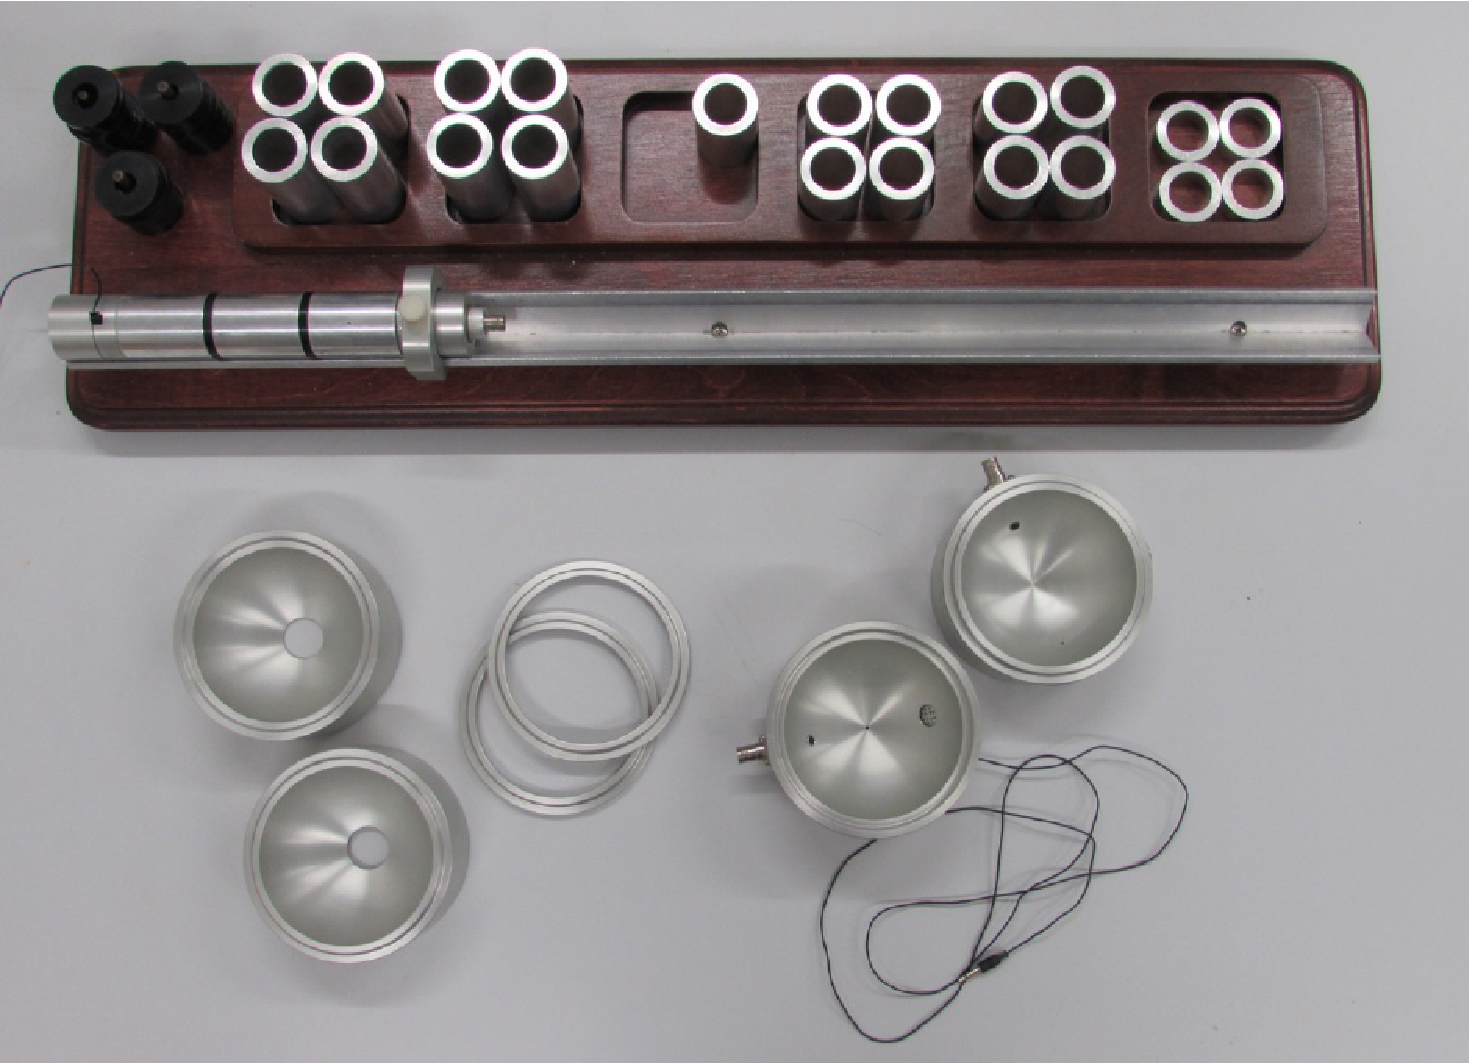
\includegraphics[width=0.6\textwidth]{figure/Aufbau.pdf}
    \caption{In dieser Abbildung sind die Baukomponenten der einzelnen Versuchsteile 
    dargestellt. Im oberen Bildbereich sind die Aluminumzylinder und die 
    zugehörigen schwarzen Blenden zu sehen, darunter befindet sich die 
    Metallschiene auf der die Zylinder aufgereiht und zur Frequenzmessung 
    positioniert werden können. Im unteren Bildbereich sind rechts die beiden 
    Hälften des Kugelresonators mit Lautsprecher und Mikrofon, mittig die 
    Zwischenringe und links die beiden Halbkugeln mit Öffnungen abgebildet 
    \cite{sample}.}
\end{figure}
\newpage

\section{Versuchsdurchführung}
\label{sec:Versuchsdurchführung}

Dieser Versuch ist in vier Messsegmente gegliedert.
Zunächst wird die Resonanzfrequenz von hintereinander gereihten Aluminiumzylindern 
verschiedener Anzahl 
gesucht. Danach werden Wasserstoffatom und das Wasserstoffmolekül aus den zugehörigen 
Bauteilen (siehe Kaptilel \ref{sec:Versuchsaufbau}) zusammengesetzt, um weitere
Frequenzspektren aufzunehmen und später mit Kugelflächenfunktionen vergleichen zu können.
Als letztes werden bis zu 12 Aluminiumzylinder aufgereiht, wobei sich  
Blenden mit unterschiedlichem Durchmesser zwischen ihnen befinden. Die aufgenommenen 
Frequenzspektren werden mit Frequenzen deren Ursprung Schwingungen in einem 
eindimensionalen Festkörper waren, in Zusammenhang gebracht.

\begin{enumerate}
    \item Vorbereitung:\\
        Als erstes wird ein Aluminiumzylinder in die Metallschiene gelegt, sodass 
        sich Mikrofon und Lautsprecher jeweils an einer Öffnung des Zylinders befinden.
        Das System wird an ein Zweikanaloszilloskop und ein Sinusgenerator angeschlossen. 
        Die Schallfrequenz wird 
        wird von $\SI{6,75}{\kilo\hertz}$ ausgehend erhöht, bis die erste und 
        zweite Resonanzfrequenz 
        erreicht wird. Beide Frequenzen werden mit der zugehörigen Schalldruckamplitude und 
        Phasenverschiebung notiert. Die Messung wird danach für zwei bis sechs Zylinder 
        wiederholt. Die Messreihe wird für jede Zylinderanzahl ein weiteres Mal wiederholt,
        während ein Computer mit dem Programm SpectrumSLC anstelle des Oszilloskops zur Visualiesierung 
        des Frequenzspektrums an 
        die Metallschiene angeschlossen wird. 
    \item Wasserstoffatom:\\
        Das Wasserstoffatommodel wird so zusammengesetzt, dass sich Lautsprecher und Microfon
        in einem Winkel von $\num{180}°$ zueinander befinden. 
        Dann wird mit ein sinusgenerator und ein Zweikanaloszilloskop angeschlossen. 
        Während der Frequenzbereich zwischen $\SI{100}{\hertz}$ und $\SI{100}{\kilo\hertz}$
        schrittweise abgelaufen wird, werden die Amplituden, Physenverschiebungen und 
        Resonanzfrequenzen bis zur elften ordnung aufgeschrieben. 
        Die Messung wird mit einem Computer im Programm SpectrumSLC für ein 
        kontinuilierliches Frequenzspektrum im seben Bereich wiederholt.
        Danach wird der Winkel zwischen Lautsprecher und Mikrofon in $\num{10}°$
        Schritten zwischen $\num{0}°$ und $\num{180}°$ verstellt, während
        für die zweite, vierte und sechste Resonanfrequenz Amplitude aufgenommenen
        wird.
        Für die folgenden Messungen wird
        die Signalfrequenz konstant auf $\SI{2,3}{\kilo\hertz}$ und der Winkel 
        zunächst auf $\num{180}°$
        eingestellt. Dabei wird für jeden Zwischenringe und jede mögliche Kombination 
        aus Zwischenringen ein Frequenzspektrum aufgenommen.
        Während der $\SI{9}{\milli\meter}$ Zwischenring eingespannt ist, wird zusätlzich 
        eine Amplitudenverteilung in Abhängigkeit des Winkels zwischen Mikrofon und 
        Lautsprecher aufgenommenen. Dabei wird erneut der Bereich zwischen 
        $\num{0}°$ und $\num{180}°$ in $\num{10}°$ Schritten abgelaufen.
        \newpage
    \item Wasserstoffmolekül:\\
        Um das Wasserstoffmolekül aufzubauen werden zwischen die Halbkugeln des 
        Wasserstoffatoms zwei Halbkugeln mit einer Öffnung geschraubt, sodass sich 
        zwei Kugeln ergeben, die durch eine Öffnung miteinander verbunden sind.
        In diese Öffnung wird für die erste Messung eine Blende mit einem 
        Durchmesser von $\SI{10}{\milli\meter}$ und für die zweite Messung eine 
        Blende mit dem Durchmesser $\SI{16}{\milli\meter}$ eingespannt.
        Dann wird ein Frequenzspektrum bei einer Resonanzfrequenz von 
        $\SI{2,3}{\kilo\hertz}$ aufgenommen. 
        Bei der $\SI{16}{\milli\meter}$ Blende wird zusätzlich eine
        Winkelverteilung in analogen Schritten bezüglich der Durchführung
        zum Wasserstoffatom aufgenommen.
    \item eindimensionaler Festkörper:\\
        Für diesen Versuchsteil wird zunächst das Frequenzspektrum für einen 
        $\SI{50}{\milli\meter}$ Zylinder aufgenommen. Daraufhin wird eine 
        $\SI{13}{\milli\meter}$ Blende und ein weiterer Zylinder angehangen, sodass 
        ein neues Frequenzspektrum aufgenommen werden kann. Das Verfahren wird 
        solange wiederholt bis eine Kette von $\num{12}$ Zylindern und $\num{11}$
        Blenden erreicht ist. Danach wird einer der Zylinder erst durch einen 
        $\SI{75}{\milli\meter}$ Zylinder und dann durch zwei $\SI{12,5}{\milli\meter}$
        ersetzt. Beide Male wird das zugehörige Spektrum aufgenommen.
        Das letzte Frequenzspektrum wird ebenfalls für $\num{12}$ Zylindern und $\num{11}$
        Blenden aufgenommen, wobei alle Zylinder eine Länge von $\SI{50}{\milli\meter}$
        haben, die Blenden jedoch abwechselnd einen Durchmesser von
        $\SI{13}{\milli\meter}$ und $\SI{16}{\milli\meter}$ aufweisen müssen.
\end{enumerate}

\cite{sample}
\newpage